\documentclass{beamer}
\usepackage{hyperref}
\usepackage[T1]{fontenc}

% other packages
\usepackage{latexsym,amsmath,xcolor,multicol,booktabs,calligra}
\usepackage{graphicx,pstricks,listings,stackengine}

% dummy text; remove it when working on this template
\usepackage{lipsum}

\usepackage{tikz}

\author{Vasileios Dimitriou}

\title{Diploma Thesis}

\subtitle{Investigation of Machine Vibration Analysis System Design}
\institute{
	Department of Electrical and Software Engineering \\
	University of Thessaly
}
\date{\small September, 2025}
\usepackage{Ritsumeikan}

% defs
\def\cmd#1{\texttt{\color{red}\footnotesize $\backslash$#1}}
\def\env#1{\texttt{\color{blue}\footnotesize #1}}
\definecolor{deepblue}{rgb}{0,0,0.5}
\definecolor{deepred}{RGB}{153,0,0}
\definecolor{deepgreen}{rgb}{0,0.5,0}
\definecolor{halfgray}{gray}{0.55}

\lstset{
	basicstyle=\ttfamily\small,
	keywordstyle=\bfseries\color{deepblue},
	emphstyle=\ttfamily\color{deepred},    % Custom highlighting style
	stringstyle=\color{deepgreen},
	numbers=left,
	numberstyle=\small\color{halfgray},
	rulesepcolor=\color{red!20!green!20!blue!20},
	frame=shadowbox,
}


\begin{document}
	
	\begin{frame}
		\titlepage
		\vspace*{-0.6cm}
		\begin{figure}[htpb]
			\begin{center}
				
\includegraphics[keepaspectratio, scale=0.14]{pic/uchicago.png}
			\end{center}
		\end{figure}
	\end{frame}
	
	\begin{frame}    
		\tableofcontents[sectionstyle=show,
		subsectionstyle=show/shaded/hide,
		subsubsectionstyle=show/shaded/hide]
	\end{frame}
	
	\section{Introduction}
	
	\begin{frame}{Predictive Maintenance and Condition Monitoring}
		\begin{figure}[h]  
			\centering  
			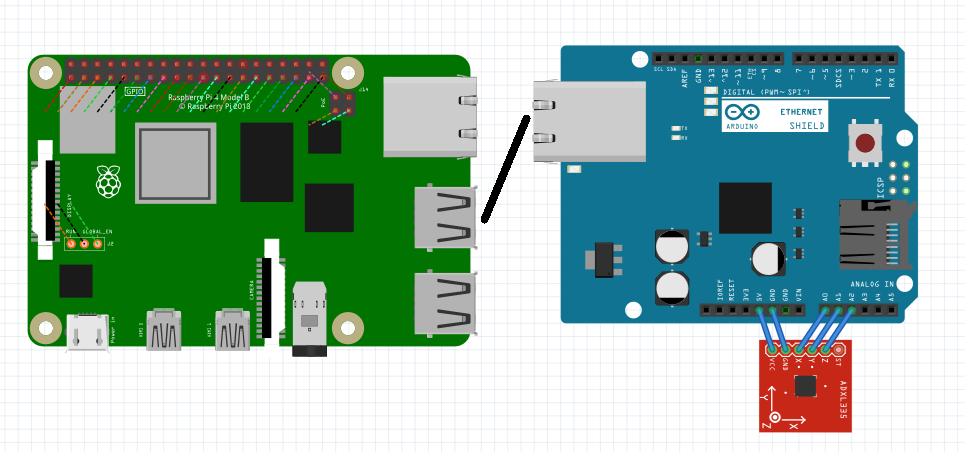
\includegraphics[width=\linewidth]{images/System.png}  
			\caption{Hardware architecture with signal flow.}  
			\label{fig:System}  
		\end{figure}
	\end{frame}
	
	\begin{frame}{Predictive Maintenance and Condition Monitoring}
	    \begin{itemize}[<+-| alert@+>]
			\item Development of a low-cost embedded system for predictive maintenance [see Figure \ref{fig:System}].
			\item Development of software for data acquisition and transmission from Arduino UNO R3 to Raspberry Pi 4.
			\item Development of software for FFT-based spectral analysis software on Raspberry Pi 4 for frequency-domain feature extraction.
			\item Development of a secure, authenticated API client for structured data transmission from Raspberry Pi 4 to Supabase.
			\item Implementation of a Vercel API endpoint that fetches measurement data from Supabase database.
			\item Development of a React frontend that requests and visualizes data from the Vercel API.
		\end{itemize}
	\end{frame}

	
	
	
	
	
	
	
	
	
	
	\section{Background}
	
	
	\subsection{Model Background}
	\begin{frame}{Equipment Operational Anomalies}
	\begin{figure}[h]
		\centering
		\resizebox{\columnwidth}{!}{
			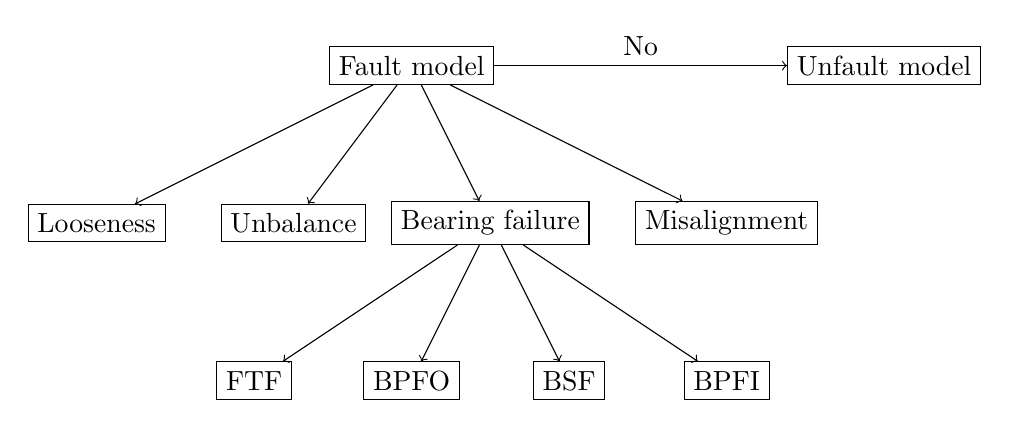
\begin{tikzpicture}[node distance=1.5cm]
				\node (box1) [draw, rectangle] at (0,0) {Unfault model};
				\node (box2) [draw, rectangle, left of=box1, node distance=6cm] {Fault model};
				\node (box3) [draw, rectangle] at (-7.5,-2) {Unbalance};
				\node (box4) [draw, rectangle] at (-2,-2) {Misalignment};
				\node (box5) [draw, rectangle] at (-5,-2) {Bearing failure};
				\node (box6) [draw, rectangle] at (-10,-2) {Looseness};
				\node (box7) [draw, rectangle] at (-6,-4) {BPFO};
				\node (box8) [draw, rectangle] at (-2,-4) {BPFI};
				\node (box9) [draw, rectangle] at (-4,-4) {BSF};
				\node (box10) [draw, rectangle] at (-8,-4) {FTF};
				
				% Arrows with labels
				\draw[->] (box2) -- node[midway, above] {No} (box1);
				\draw[->] (box2) -- (box3);
				\draw[->] (box2) -- (box4);
				\draw[->] (box2) -- (box5);
				\draw[->] (box2) -- (box6);
				\draw[->] (box5) -- (box7);
				\draw[->] (box5) -- (box8);
				\draw[->] (box5) -- (box9);
				\draw[->] (box5) -- (box10);
			\end{tikzpicture}
		}
			\caption{Fault tree analysis diagram showing the relationship between machine conditions and specific fault frequencies.} \label{fig:faultTree}
	\end{figure}
	\end{frame}
	
	





	
	
	\section{Engineering and Design}
	\begin{frame}
		\frametitle{System Architecture and Dataflow}
		\begin{figure}[h]  
			\centering  
			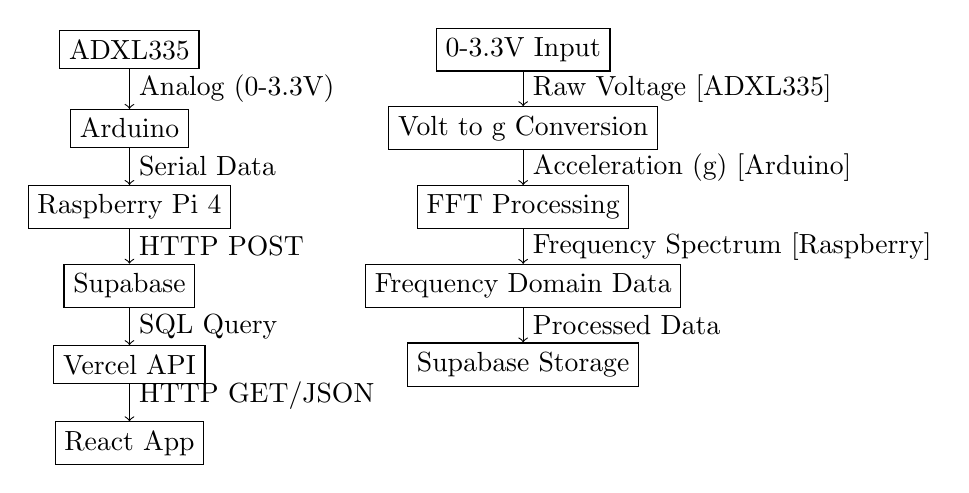
\begin{tikzpicture}[node distance=1cm]
				% Architecture Diagram (Left)
				\node (sensor) [draw, rectangle] {ADXL335};  
				\node (arduino) [draw, rectangle, below of=sensor] {Arduino};  
				\node (rpi) [draw, rectangle, below of=arduino] {Raspberry Pi 4};  
				\node (supabase) [draw, rectangle, below of=rpi] {Supabase};  
				\node (vercel) [draw, rectangle, below of=supabase] {Vercel API};  
				\node (react) [draw, rectangle, below of=vercel] {React App};  
				
				\draw[->] (sensor) -- node[right] {Analog (0-3.3V)} (arduino);  
				\draw[->] (arduino) -- node[right] {Serial Data} (rpi);  
				\draw[->] (rpi) -- node[right] {HTTP POST} (supabase);  
				\draw[->] (supabase) -- node[right] {SQL Query} (vercel);  
				\draw[->] (vercel) -- node[right, pos=0.3] {HTTP GET/JSON} (react);
				
				% Data Transformation Diagram (Right)
				\begin{scope}[xshift=5cm]
					\node (voltage) [draw, rectangle] {0-3.3V Input};
					\node (conversion) [draw, rectangle, below of=voltage] {Volt to g Conversion};
					\node (fft) [draw, rectangle, below of=conversion] {FFT Processing};  % Fixed reference
					\node (freqDomain) [draw, rectangle, below of=fft] {Frequency Domain Data};
					\node (database) [draw, rectangle, below of=freqDomain] {Supabase Storage};
					
					\draw[->] (voltage) -- node[right] {Raw Voltage [ADXL335]} (conversion);
					\draw[->] (conversion) -- node[right] {Acceleration (g) [Arduino]} (fft);  % Fixed target
					\draw[->] (fft) -- node[right] {Frequency Spectrum [Raspberry]} (freqDomain);
					\draw[->] (freqDomain) -- node[right] {Processed Data} (database);
				\end{scope}
			\end{tikzpicture}  
			\caption{Complete system architecture and data flow and transformation pipeline from physical sensor to web visualization dashboard.}
			\label{fig:dataflow}  
		\end{figure}
	\end{frame}	
	
	
	
	
	
	
	

	\section{Implementation}
	\subsection{Fault Type Classification}
	\begin{frame}{Fault Type Classification}
	\begin{figure}[h]
		\centering
		\resizebox{\columnwidth}{!}{
			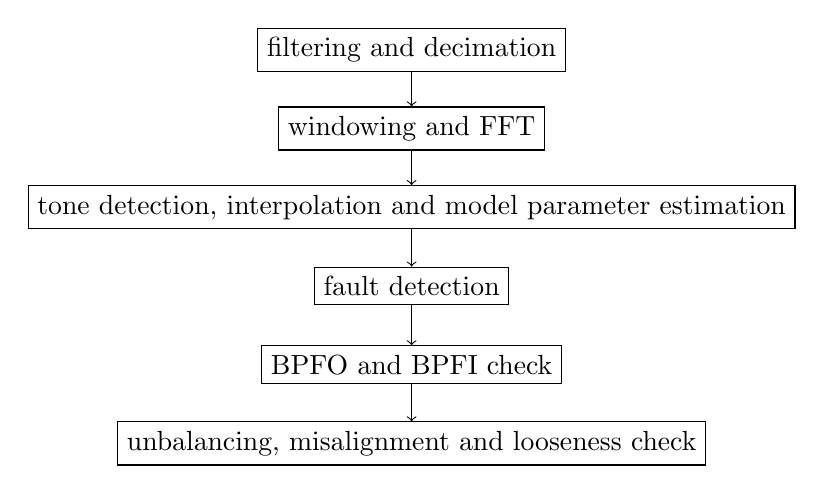
\begin{tikzpicture}
				\node (box1) [draw, rectangle] at (0,0) {filtering and decimation};
				\node (box2) [draw, rectangle, below of=box1, node distance=1cm] {windowing and FFT};
				\node (box3) [draw, rectangle, below of=box2, node distance=1cm] {tone detection, interpolation and model parameter estimation};
				\node (box4) [draw, rectangle, below of=box3, node distance=1cm] {fault detection};
				\node (box5) [draw, rectangle, below of=box4, node distance=1cm] {BPFO and BPFI check};
				\node (box6) [draw, rectangle, below of=box5, node distance=1cm] {unbalancing, misalignment and looseness check};
				
				% Arrows
				\draw[->] (box1) -- (box2);
				\draw[->] (box2) -- (box3);
				\draw[->] (box3) -- (box4);
				\draw[->] (box4) -- (box5);
				\draw[->] (box5) -- (box6);
			\end{tikzpicture}
		}
		\caption{The series of checks carried out by the algorithm}
		\label{fig:checks}
	\end{figure}	
	\end{frame}
	
	\subsection{Power Spectrum Density calculation}
	\begin{frame}{Power Spectrum Density calculation}
	Power Spectrum Density Threshold Calculation:
	
	\[
	\text{PSD} = \frac{(\text{Power Spectrum})^2}{\Delta f \times \text{Noise Power Bandwidth of Window}}
	\]
	Where: 
	\begin{itemize}
		\item Power spectrum is calculated by taking the average of the magnitude squared of multiple frequency spectra \[ PS = \frac{2 \times \text{X}^2}{N^2} \]
		\item \[ \Delta f  = \frac{f_{s}}{N} \] is the frequency resolution 
		\item Noise Power Bandwidth of Window is a correction factor for the rectangular window
	\end{itemize}
	\end{frame}
	
	\begin{frame}{Power Spectrum Density calculation}
	\begin{figure}[h]
		\centering
		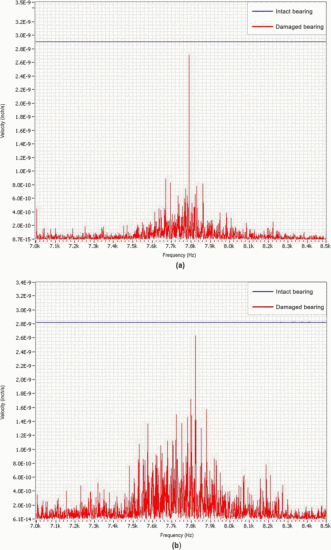
\includegraphics[width=0.3\linewidth]{images/PSDCombinedloaded.png}
		\caption{Combination of all the aforementioned faults (inner case, outer case and bearing ball fault) \cite{Azeem2019}.}
		\label{fig:PSDCombinedloaded}
	\end{figure}
	\end{frame}
	
	\subsection{Dynamic signal stability analysis}
	\begin{frame}{Dynamic signal stability analysis}
	\begin{figure}[h]
		\centering
		\resizebox{\columnwidth}{!}{
			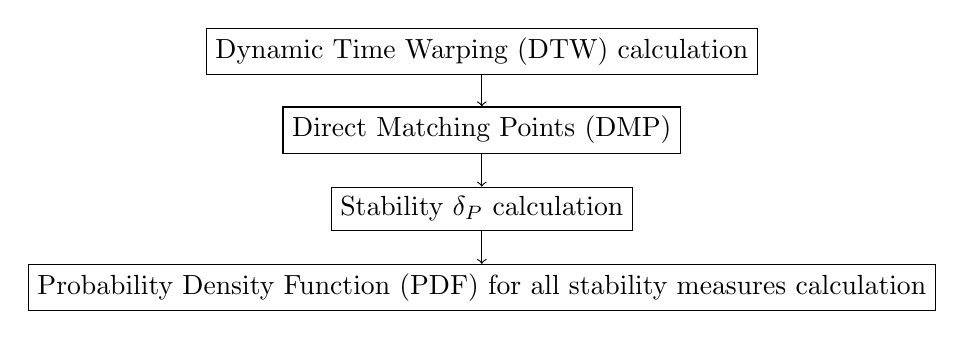
\begin{tikzpicture}
				\node (box1) [draw, rectangle] at (0,0) {Dynamic Time Warping (DTW) calculation};
				\node (box2) [draw, rectangle, below of=box1, node distance=1cm] {Direct Matching Points (DMP)};
				\node (box3) [draw, rectangle, below of=box2, node distance=1cm] {Stability $\delta_P$ calculation};
				\node (box4) [draw, rectangle, below of=box3, node distance=1cm] {Probability Density Function (PDF) for all stability measures calculation};
				
				
				% Arrows
				\draw[->] (box1) -- (box2);
				\draw[->] (box2) -- (box3);
				\draw[->] (box3) -- (box4);
				
			\end{tikzpicture}
		}
		\caption{The series of checks carried out by the algorithm}
		\label{fig:stabilityprocessflowdiagram}
	\end{figure}
	\end{frame}
	
	\subsection{Vibration Spectrum and phase analysis}
	\begin{frame}{ Vibration Spectrum and phase analysis}
	\begin{figure}[h]
		\centering
		\resizebox{\columnwidth}{!}{
			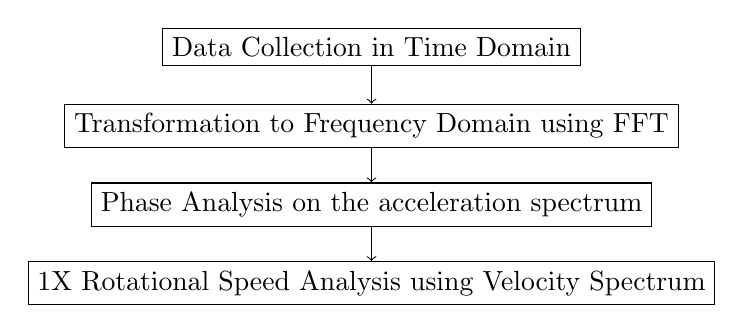
\begin{tikzpicture}
				\node (box1) [draw, rectangle] at (0,0) {Data Collection in Time Domain};
				\node (box2) [draw, rectangle, below of=box1, node distance=1cm] {Transformation to Frequency Domain using FFT};
				\node (box3) [draw, rectangle, below of=box2, node distance=1cm] {Phase Analysis on the acceleration spectrum};
				\node (box4) [draw, rectangle, below of=box3, node distance=1cm] {1X Rotational Speed Analysis using Velocity Spectrum};
				
				
				% Arrows
				\draw[->] (box1) -- (box2);
				\draw[->] (box2) -- (box3);
				\draw[->] (box3) -- (box4);
				
			\end{tikzpicture}
		}
		\caption{The series of checks carried out by the algorithm}
		\label{fig:specandphase}
	\end{figure}
	\end{frame}
	
	
	
	
	
	\subsection{Incipient SVM on time-domain}
		\begin{frame}{Incipient SVM Fault Detection Model and Anomaly Detection Model on time-domain dataset}	
		\begin{figure}[h]
			\centering
			\resizebox{\columnwidth}{!}{
				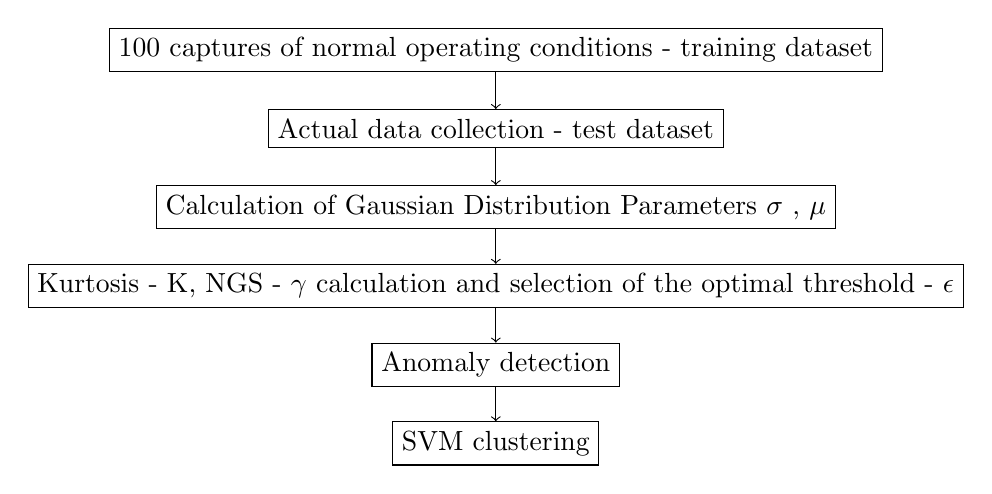
\begin{tikzpicture}
					\node (box1) [draw, rectangle] at (0,0) {100 captures of normal operating conditions - training dataset};
					\node (box2) [draw, rectangle, below of=box1, node distance=1cm] {Actual data collection - test dataset};
					\node (box3) [draw, rectangle, below of=box2, node distance=1cm] {Calculation of Gaussian Distribution Parameters $\sigma$ , $\mu$};
					\node (box4) [draw, rectangle, below of=box3, node distance=1cm] {Kurtosis - K, NGS - $\gamma$ calculation and selection of the optimal threshold - $\epsilon$};
					\node (box5) [draw, rectangle, below of=box4, node distance=1cm] {Anomaly detection};
					\node (box6) [draw, rectangle, below of=box5, node distance=1cm] {SVM clustering};
					
					% Arrows
					\draw[->] (box1) -- (box2);
					\draw[->] (box2) -- (box3);
					\draw[->] (box3) -- (box4);
					\draw[->] (box4) -- (box5);
					\draw[->] (box5) -- (box6);
				\end{tikzpicture}
			}
			\caption{Incipient SVM Model}
			\label{fig:svm}
		\end{figure}	
	\end{frame}


	\subsection{Incipient fault detection with one-class v-SVM algorithm}
	\begin{frame}{Incipient fault detection with one-class v-SVM algorithm}	
	\begin{figure}[h]
		\centering
		\resizebox{\columnwidth}{!}{
			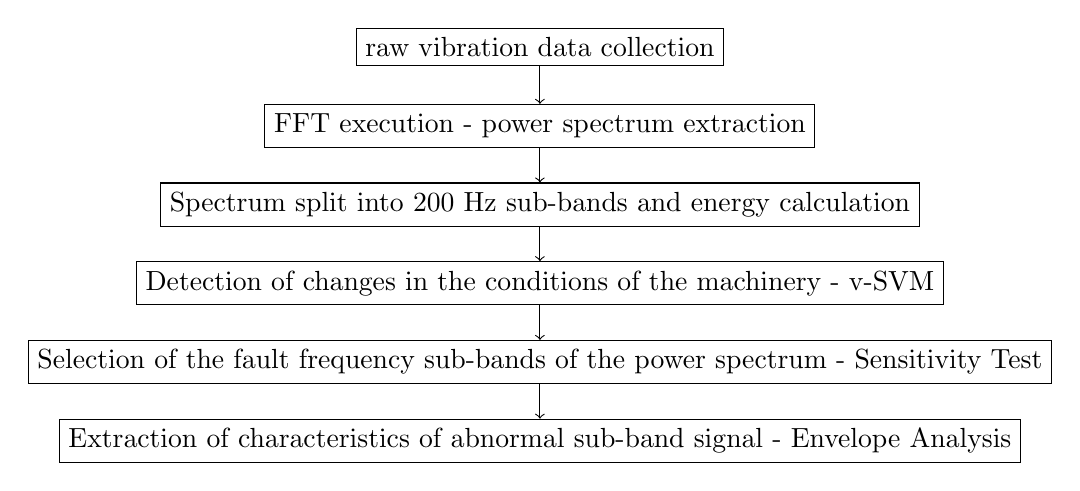
\begin{tikzpicture}
				\node (box1) [draw, rectangle] at (0,0) {raw vibration data collection};
				\node (box2) [draw, rectangle, below of=box1, node distance=1cm] {FFT execution - power spectrum extraction};
				\node (box3) [draw, rectangle, below of=box2, node distance=1cm] {Spectrum split into 200 Hz sub-bands and energy calculation};
				\node (box4) [draw, rectangle, below of=box3, node distance=1cm] {Detection of changes in the conditions of the machinery - v-SVM};
				\node (box5) [draw, rectangle, below of=box4, node distance=1cm] {Selection of the fault frequency sub-bands of the power spectrum - Sensitivity Test};
				\node (box6) [draw, rectangle, below of=box5, node distance=1cm] {Extraction of characteristics of abnormal sub-band signal - Envelope Analysis};
				
				% Arrows
				\draw[->] (box1) -- (box2);
				\draw[->] (box2) -- (box3);
				\draw[->] (box3) -- (box4);
				\draw[->] (box4) -- (box5);
				\draw[->] (box5) -- (box6);
			\end{tikzpicture}
		}
		\caption{Architecture of anomaly detection frequency sub-band \cite{Francos2013}}
		\label{fig:v-svm}
	\end{figure}
	\end{frame}
	
	
	\subsection{Real-time fault detection set-up with SVM algorithm}
	\begin{frame}{Real-time fault detection set-up with SVM algorithm}	
	\begin{figure}[h]
		\centering
		\resizebox{\columnwidth}{!}{
			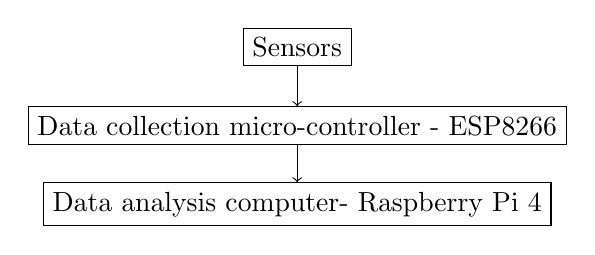
\begin{tikzpicture}
				\node (box1) [draw, rectangle] at (0,0) {Sensors};
				\node (box2) [draw, rectangle, below of=box1, node distance=1cm] {Data collection micro-controller - ESP8266};
				\node (box3) [draw, rectangle, below of=box2, node distance=1cm] {Data analysis computer- Raspberry Pi 4}; 
				
				% Arrows
				\draw[->] (box1) -- (box2);
				\draw[->] (box2) -- (box3);
				
			\end{tikzpicture}
		}
		\caption{Architecture of anomaly detection frequency sub-band \cite{Raman2023}}
		\label{fig:sensors}
	\end{figure}
	\end{frame}
	
	
	
	\subsection{Backpropagation Neural Network}
	\begin{frame}{Backpropagation Neural Network}	
	\begin{figure}[h]
		\centering
		\resizebox{\columnwidth}{!}{
			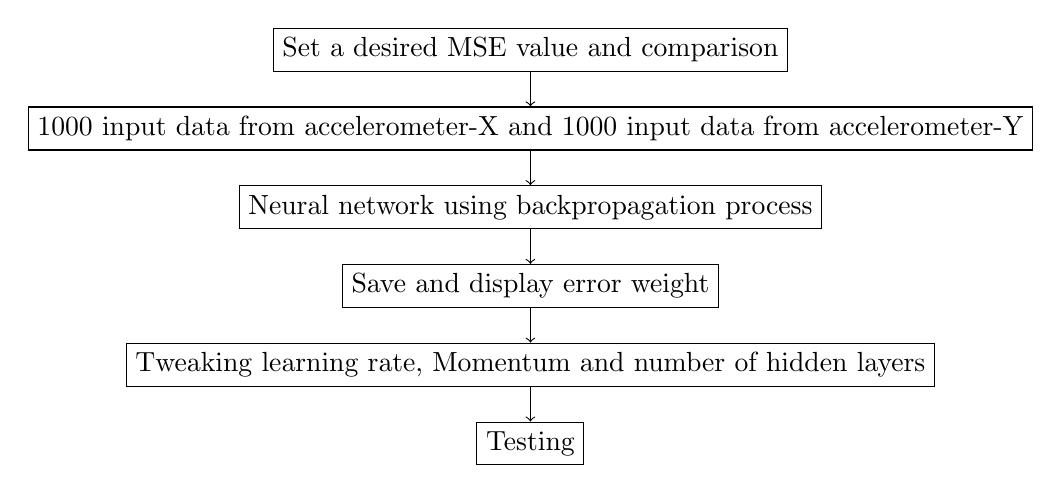
\begin{tikzpicture}
				\node (box1) [draw, rectangle] at (0,0) {Set a desired MSE value and comparison};
				\node (box2) [draw, rectangle, below of=box1, node distance=1cm] {1000 input data from accelerometer-X and 1000 input data from accelerometer-Y};
				\node (box3) [draw, rectangle, below of=box2, node distance=1cm] {Neural network using backpropagation process}; 
				\node (box4) [draw, rectangle, below of=box3, node distance=1cm] {Save and display error weight};
				\node (box5) [draw, rectangle, below of=box4, node distance=1cm] {Tweaking learning rate, Momentum and number of hidden layers};
				\node (box6) [draw, rectangle, below of=box5, node distance=1cm] {Testing};
				
				% Arrows
				\draw[->] (box1) -- (box2);
				\draw[->] (box2) -- (box3);
				\draw[->] (box3) -- (box4);
				\draw[->] (box4) -- (box5);
				\draw[->] (box5) -- (box6);
			\end{tikzpicture}
		}
		\caption{Flowchart for the Backpropagation-Neural Network (B-NN) training and testing \cite{Kuspijani2020}.}
		\label{fig:BNNflowchart}
	\end{figure}
	\end{frame}
	
	
	
	\section{Results}
	\begin{frame}
		\begin{itemize}
			\item \textbf{Vibration Analysis Techniques:} Wide variety including time-domain and frequency-domain analysis.
			
			\item \textbf{Fault Detection Algorithms:} Use parameters or thresholds for classification, highly effective for assessing machinery health. Dynamic signal stability analysis is a standout tool.
			
			\item \textbf{Machine Learning Anomaly Detection:} Can be combined with root algorithms, focus on continuous monitoring and past data analysis in specific application contexts.
		\end{itemize}
	\end{frame}
	
	

	\section{Conclusions}
	\begin{frame}
		\begin{itemize}
			\item \textbf{Vibration Analysis Techniques:} Wide variety including time-domain and frequency-domain analysis.
			
			\item \textbf{Fault Detection Algorithms:} Use parameters or thresholds for classification, highly effective for assessing machinery health. Dynamic signal stability analysis is a standout tool.
			
			\item \textbf{Machine Learning Anomaly Detection:} Can be combined with root algorithms, focus on continuous monitoring and past data analysis in specific application contexts.
		\end{itemize}
	\end{frame}
	
	
	
	
	
	
%	
%	
%	
%	\section{References}
%	
%	\begin{frame}[allowframebreaks]
%		\renewcommand{\refname}{References} 
%		\bibliographystyle{ieeetr}
%		\bibliography{references}
%		\nocite{*} % used here because no citation happens in slides
%		% if there are too many try use：
%		% \tiny\bibliographystyle{alpha}
%	\end{frame}
%	
%	
%	\begin{frame}
%		\begin{center}
%			{\Huge\calligra Thank You}
%		\end{center}
%	\end{frame}
	
\end{document}